%% FullCourse_10Lecs -- Lecture 10, Topic 10.3: Case Study 2 --- MEPS Uninsurance
%% Source: ./archive_pre_split/Lec10_Case_Studies_v2.tex (section 3)
%% Pass B: layer in refinements from
%%         ../../MiniCourse_8hr/Slides/Module4_Agentic_AI/M4_T6_Case_LaborMarket.tex
%% Pass B ports: Census CPS ASEC validation framing, weighted statistics
%%         emphasis (estimand, three-reason bias argument, sanity-check
%%         pyramid), agentic-pipeline diagram, sub-agent pattern.

%% Shared preamble for the FullCourse_10Lecs topic decks.
%%
%% Each topic .tex \input's this file, then defines its own \title, \date
%% override (if any), \graphicspath, and \begin{document}.
%%
%% Reconstructed verbatim from the inlined copy preserved in
%% Lec10_Case_Studies/Lec10_T8_Case6_DeepRamsey.tex (lines 23-190), which is
%% explicitly annotated there as "from ../shared_preamble.tex, copied verbatim".
%% Base preamble matches MiniCourse_8hr/Slides/shared_preamble.tex; this version
%% additionally provides \sectiondivider, the conceptbox/cautionbox/examplebox/
%% takeawaybox tcolorboxes, and \compacttables used across the split decks.

\documentclass[10pt,english,aspectratio=169]{beamer}

\usepackage{ae,aecompl}
\usepackage[T1]{fontenc}
\usepackage{textcomp}
\usepackage[utf8]{inputenc}
\usepackage{babel}
\usepackage{datetime2}

\setcounter{secnumdepth}{3}
\setcounter{tocdepth}{3}

\usepackage{amsmath, amssymb, amsthm, graphicx}
\usepackage{booktabs, multirow}
\usepackage{tikz}
\usepackage{pgfplots}
\pgfplotsset{compat=1.16}
\usepackage[most]{tcolorbox}
\tcbuselibrary{skins, breakable, theorems}
\usepackage{listings}
\usepackage{xcolor}

\lstset{
  basicstyle=\ttfamily\small,
  keywordstyle=\color{blue!80!black}\bfseries,
  commentstyle=\color{green!50!black}\itshape,
  stringstyle=\color{orange!80!black},
  backgroundcolor=\color{gray!8},
  frame=single,
  rulecolor=\color{gray!40},
  breaklines=true,
  showstringspaces=false,
  numbers=none,
}

\lstdefinestyle{pythonstyle}{
    language=Python,
    basicstyle=\ttfamily\footnotesize,
    keywordstyle=\color{blue!80!black}\bfseries,
    commentstyle=\color{green!50!black}\itshape,
    stringstyle=\color{orange!80!black},
    frame=single,
    breaklines=true,
    showstringspaces=false,
    numbers=left,
    numbersep=5pt,
    numberstyle=\tiny\color{gray},
    backgroundcolor=\color{gray!8},
    rulecolor=\color{gray!40}
}

\ifx\hypersetup\undefined
  \AtBeginDocument{%
    \hypersetup{bookmarks=false,breaklinks=true,pdfborder={0 0 0},colorlinks=true,
      linkcolor=DarkText,urlcolor=RedTitle}%
  }
\else
  \hypersetup{bookmarks=false,breaklinks=true,pdfborder={0 0 0},colorlinks=true,
    linkcolor=DarkText,urlcolor=RedTitle}%
\fi

\makeatletter
\newcommand\makebeamertitle{%
  \begin{frame}[plain]
    \vspace*{1.0cm}
    \centering
    {\usebeamerfont{title}\usebeamercolor[fg]{title}\inserttitle\par}
    \vspace{1.0cm}
    {\usebeamerfont{author}\usebeamercolor[fg]{author}\insertauthor\par}
    \vspace{0.2cm}
    {\usebeamerfont{date}\usebeamercolor[fg]{date}\insertdate\par}
  \end{frame}}%
\AtBeginDocument{%
  \let\origtableofcontents=\tableofcontents
  \def\tableofcontents{\@ifnextchar[{\origtableofcontents}{\gobbletableofcontents}}
  \def\gobbletableofcontents#1{\origtableofcontents}%
}

\usetheme{metropolis}
\usefonttheme{professionalfonts}

\definecolor{LightGray}{RGB}{230,230,230}
\definecolor{RedTitle}{RGB}{0,0,200}
\definecolor{VeryLightGray}{RGB}{245,245,245}
\definecolor{DarkText}{RGB}{0,0,0}

\setbeamercolor{background canvas}{bg=white}
\setbeamercolor{title}{fg=RedTitle}
\setbeamercolor{author}{fg=DarkText}
\setbeamercolor{date}{fg=DarkText}
\setbeamercolor{frametitle}{bg=VeryLightGray,fg=DarkText}
\setbeamercolor{normal text}{fg=DarkText}
\setbeamerfont{title}{size=\large}

\setbeamersize{text margin left=5mm, text margin right=5mm}
\addtobeamertemplate{frametitle}{}{\vspace{-0.5em}}
\newcommand{\reducevspace}{\vspace{-0.5cm}}

% Shared section divider and box styles for split topic decks.
\newcommand{\sectiondivider}[2]{%
\begin{frame}[plain,noframenumbering]
\begin{center}
\vfill
{\Large\textbf{#1}\par}
\vspace{0.35cm}
{\normalsize #2\par}
\vfill
\end{center}
\end{frame}
}

\newtcolorbox{conceptbox}[1][]{
  colback=blue!3,
  colframe=RedTitle!55,
  boxrule=0.35mm,
  arc=1mm,
  left=2mm,
  right=2mm,
  top=1mm,
  bottom=1mm,
  #1
}
\newtcolorbox{cautionbox}[1][]{
  colback=red!3,
  colframe=red!50!black,
  boxrule=0.35mm,
  arc=1mm,
  left=2mm,
  right=2mm,
  top=1mm,
  bottom=1mm,
  #1
}
\newtcolorbox{examplebox}[1][]{
  colback=green!3,
  colframe=green!45!black,
  boxrule=0.35mm,
  arc=1mm,
  left=2mm,
  right=2mm,
  top=1mm,
  bottom=1mm,
  #1
}
\newtcolorbox{takeawaybox}[1][]{
  colback=VeryLightGray,
  colframe=RedTitle!55,
  boxrule=0.35mm,
  arc=1mm,
  left=2mm,
  right=2mm,
  top=1mm,
  bottom=1mm,
  #1
}
\newcommand{\compacttables}{\renewcommand{\arraystretch}{1.15}}

\setbeamertemplate{navigation symbols}{}
\setbeamertemplate{footline}{%
  \hfill%
  \usebeamercolor[fg]{page number in head/foot}%
  \usebeamerfont{page number in head/foot}%
  \insertframenumber\,/\,\inserttotalframenumber\kern1em\vskip2pt%
}

\makeatother

\author{Zhigang Feng}
% "date with time": compile timestamp so each build is identifiable.
\date{\today\ \DTMcurrenttime}


% Suppress redundant auto-generated metropolis section page; \sectiondivider frames are the dividers we keep.
\metroset{sectionpage=none}

\graphicspath{{./pic/}{./figures/}{./Exercise10_ES_Fellows/plots/}{../../MiniCourse_8hr/Slides/Module4_Agentic_AI/pic/}{../}}

\usetikzlibrary{positioning,arrows.meta,shapes,calc,fit,backgrounds}

\lstdefinestyle{markdownstyle}{
    basicstyle=\ttfamily\footnotesize,
    frame=single,
    rulecolor=\color{gray!40},
    backgroundcolor=\color{gray!8},
    breaklines=true,
    showstringspaces=false,
    numbers=none,
}

\title[AI for Econ Research]{AI for Economic Research: Dynamic Models, Language, and Agents\\
Lecture 10.3: Case Study 2 --- MEPS Uninsurance Analysis}

\begin{document}

\makebeamertitle

%=============================================================================
\begin{frame}{Topic 10.3 Agenda}
\begin{enumerate}
  \item \textbf{Case Study 2} --- agentic empirical pipeline on MEPS uninsurance data
\end{enumerate}
\end{frame}

%=============================================================================
\section{Case Study 2: MEPS Uninsurance}
%===========================================================

%===========================================================

\sectiondivider{Case Study 2}{A one-session empirical data pipeline with strong validation}

\begin{frame}{Case Study 2: The Macro Question}
\begin{tcolorbox}[colback=blue!3, colframe=RedTitle!60]
\textbf{Question:} Who is uninsured in the United States, 2000--2023, and how did the ACA change the distribution?
\end{tcolorbox}

\vspace{0.25cm}
\begin{itemize}
    \item health insurance is a major incomplete-market margin
    \item the ACA is a large social-insurance intervention
    \item the research value comes from who gained coverage, not just from the overall average
    \item this is the most economics-facing case in the lecture
\end{itemize}
\end{frame}

\begin{frame}{The Naive Baseline: 24 Files, 24 Headaches}
\begin{itemize}
    \item download 24 MEPS full-year files by hand
    \item discover that variable names are year-suffixed
    \item figure out which weight variable applies in each year
    \item merge everything and hope the crosswalk is right
\end{itemize}

\vspace{0.3cm}
\textbf{Where this breaks:}
\begin{enumerate}
    \item silent crosswalk mistakes
    \item dropped survey weights
    \item inconsistent file formats
    \item wrong figure even though the code runs
\end{enumerate}
\end{frame}

\begin{frame}{Why This Stays Ad Hoc Instead of Becoming a Skill}
\begin{columns}[T]
\begin{column}{0.48\textwidth}
\textbf{Skill-like features}
\begin{itemize}
    \item multi-step pipeline
    \item explicit validation
    \item repeated checks
\end{itemize}
\end{column}
\begin{column}{0.48\textwidth}
\textbf{Why still ad hoc}
\begin{itemize}
    \item single research question
    \item only three prompts
    \item interactive refinement of plots
    \item workflow is useful but not yet a reusable product
\end{itemize}
\end{column}
\end{columns}

\vspace{0.3cm}
\textbf{Case 2 verdict:} this is a structured session, not a reusable skill.
\end{frame}

\begin{frame}[fragile]{The 3-Prompt Architecture}
\begin{lstlisting}[style=pythonstyle, language={}, basicstyle=\ttfamily\scriptsize, numbers=none]
Prompt A: download, parse, and harmonize MEPS files
Prompt B: compute weighted uninsurance rates by group
Prompt C: generate publication-quality figures and annotations
\end{lstlisting}

\vspace{0.25cm}
\begin{itemize}
    \item Phase A builds infrastructure
    \item Phase B turns infrastructure into statistics
    \item Phase C turns statistics into economic evidence
\end{itemize}
\end{frame}

% ---- Ported from M4_T6: agentic pipeline diagram ----
\begin{frame}{The Agentic Pipeline: Spec $\to$ Extract $\to$ Verify $\to$ Iterate}
\begin{center}
\begin{tikzpicture}[
    box/.style={rectangle, draw=black, fill=VeryLightGray, rounded corners,
                minimum width=2.4cm, minimum height=0.95cm,
                text width=2.2cm, align=center, font=\footnotesize},
    arrow/.style={-{Stealth[length=2.5mm]}, thick}
]
    \node[box] (spec) {\textbf{Spec}\\question +\\weights + cuts};
    \node[box, right=0.25cm of spec] (extract) {\textbf{Extract}\\download +\\harmonize};
    \node[box, right=0.25cm of extract] (compute) {\textbf{Compute}\\weighted\\statistics};
    \node[box, right=0.25cm of compute] (verify) {\textbf{Verify}\\vs.\ Census\\CPS ASEC};
    \node[box, right=0.25cm of verify, fill=orange!15] (iterate) {\textbf{Iterate}\\figures +\\subgroups};
    \draw[arrow] (spec) -- (extract);
    \draw[arrow] (extract) -- (compute);
    \draw[arrow] (compute) -- (verify);
    \draw[arrow] (verify) -- (iterate);
\end{tikzpicture}
\end{center}

\medskip
\textbf{Where agentic AI helps:}
\begin{itemize}\itemsep0pt
    \item schema-aware extraction (year-suffixed names $\to$ harmonized panel)
    \item robust restart logic (network failures, malformed files)
    \item verification at each step (the agent compares its output to Census CPS ASEC rates)
\end{itemize}

\medskip
\textbf{Where it adds risk:} silent corruptions, version drift across reruns, IRB issues with restricted data --- mitigated by spec discipline and human checks.
\end{frame}

\begin{frame}{Phase A: What the Agent Actually Does}
\begin{itemize}
    \item discovers the AHRQ download pattern
    \item retries around 403 or parser failures
    \item builds a year-specific crosswalk
    \item standardizes the merged output into one panel
\end{itemize}

\vspace{0.25cm}
\textbf{This is the boring but decisive part.} If the infrastructure is wrong, every figure downstream is wrong in a disciplined-looking way.
\end{frame}

\begin{frame}{Schema Harmonization Is the Hard Part}
\small
\begin{tabular}{lccc}
\toprule
\textbf{Concept} & \textbf{2001} & \textbf{2014} & \textbf{2022} \\
\midrule
Insurance coverage & \texttt{INSCOV01} & \texttt{INSCOV14} & \texttt{INSCOV22} \\
Person weight & \texttt{PERWT01F} & \texttt{PERWT14F} & \texttt{PERWT22F} \\
Age & year-specific & \texttt{AGELAST} & \texttt{AGELAST} \\
\bottomrule
\end{tabular}

\vspace{0.3cm}
\begin{itemize}
    \item humans get tired and miss one mapping
    \item agents are good at repetitive lookups if you force them to save the crosswalk
    \item validation is still essential because a bad crosswalk can look plausible
\end{itemize}
\end{frame}

\begin{frame}{Weights Are Not Optional}
\[
\text{Uninsurance rate}_t \;=\;
\frac{\sum_i w_{it} \cdot \mathbf{1}[\texttt{INSCOV}_{it} = 3]}
{\sum_i w_{it}}
\]
where $w_{it}$ is the MEPS person-level survey weight.

\vspace{0.25cm}
\begin{itemize}
    \item MEPS is a complex survey, not a simple random sample
    \item unweighted rates distort the national picture
    \item the agent must identify the correct person-level weight, carry it through harmonization, and use it in every subgroup statistic
\end{itemize}

\vspace{0.25cm}
\textbf{Case 2 lesson:} a fast agent does not relieve you of basic survey-design discipline.
\end{frame}

% ---- Ported from M4_T6: why unweighted mean is biased ----
\begin{frame}{Why the Unweighted Mean Is Biased}
\small
\textbf{Three reasons MEPS \texttt{.mean()} gives the wrong national number.}
\begin{enumerate}\itemsep1pt
    \item \textbf{Oversampling.} MEPS oversamples low-income households and certain racial/ethnic groups; without weights, those groups are over-represented in the average.
    \item \textbf{Stratification.} The sample is drawn within strata; the weight reflects the inverse probability of inclusion in each stratum.
    \item \textbf{Non-response adjustment.} Final weights bake in non-response correction --- ignoring them ignores known selection.
\end{enumerate}

\vspace{0.15cm}
\textbf{For PSU/strata-aware standard errors:} use \texttt{statsmodels.stats.weightstats}, R's \texttt{survey} package, or \texttt{samplics} in Python. Point estimates are unbiased with weights alone; standard errors require the full design.

\vspace{0.15cm}
\textit{Point estimates need weights. Inference needs the survey design.}
\end{frame}

\begin{frame}{Validation: Trust But Verify (Census CPS ASEC)}
\small
\begin{tabular}{lcc}
\toprule
\textbf{Year} & \textbf{Census CPS ASEC benchmark} & \textbf{What MEPS should show} \\
\midrule
2010 & $\approx 16\%$ uninsured       & high pre-ACA uninsurance \\
2013 & $13.3\%$ uninsured             & near the pre-ACA peak \\
2016 & $8.8\%$ uninsured              & clear post-2014 decline \\
2019 & $\approx 8\%$                  & stable late-2010s level \\
2022 & $\approx 8\%$                  & still low relative to 2000s \\
\bottomrule
\end{tabular}

\vspace{0.25cm}
\textbf{The harmonization is correct if and only if independent benchmarks agree.} The verification gate is: ``does this look like the published series, year-by-year, in level and slope?''

\vspace{0.15cm}
\textbf{The economist's job:} know enough about the data that a 5\% or 25\% rate for 2013 looks obviously wrong. \textit{If verification fails, the bug is upstream --- in the crosswalk or the weighting --- not in the figure.}
\end{frame}

% ---- Ported from M4_T6: sanity-check pyramid ----
\begin{frame}{The Sanity-Check Pyramid}
\textbf{Run all four checks before any figure is rendered.}

\medskip
\begin{center}
\footnotesize
\begin{tabular}{|p{3.4cm}|p{3.9cm}|p{4.7cm}|}
\hline
\textbf{Check} & \textbf{Test} & \textbf{What a failure means} \\ \hline
1.\ Weights sum sensibly & $\sum_i w_i$ for 2013 $\approx$ US population & wrong weight column or filter \\ \hline
2.\ Overall rate matches CPS ASEC & within $\pm 1$ pp of published Census CPS ASEC & crosswalk or coding bug \\ \hline
3.\ Subgroup ordering plausible & children's rates $<$ adult rates & group definition wrong \\ \hline
4.\ Time pattern matches policy & visible drop in 2014 & year filter or weighting bug \\ \hline
\end{tabular}
\end{center}

\medskip
\textbf{Anti-pattern.} Skipping straight to plotting because the numbers ``look about right.'' One slightly off subgroup is enough to mislead a referee.

\medskip
\textit{The economist's lever: pick the four checks that, together, would catch every realistic failure mode of \emph{this} dataset.}
\end{frame}

% ---- Ported from M4_T6: sub-agent for cross-year diffing ----
\begin{frame}{Sub-Agent Pattern for Cross-Year Diffing}
\textbf{Pattern:} one agent extracts; a second \emph{verifies} the extraction is internally consistent.

\medskip
\begin{center}
\footnotesize
\begin{tabular}{|p{2.5cm}|p{3.0cm}|p{6.0cm}|}
\hline
\textbf{Sub-agent} & \textbf{Permissions} & \textbf{Job in MEPS harmonization} \\ \hline
\texttt{extractor} & READ + WRITE in \texttt{data/} & builds \texttt{crosswalk.csv} from raw files \\ \hline
\texttt{schema-reviewer} & READ-ONLY & diffs \texttt{INSCOV} categories across years; flags new codes \\ \hline
\texttt{verifier} & EXECUTE & re-runs Phase B for one canary year (2013); checks against benchmark \\ \hline
\end{tabular}
\end{center}

\medskip
\textbf{Why the separation matters.} The \texttt{extractor} is biased toward ``done.'' The \texttt{schema-reviewer} is paid to find a flaw. If \texttt{INSCOV} added a new code in some year, the diff catches it before Phase B silently buckets it as ``insured.''
\end{frame}

\begin{frame}{Figure 1: Overall Uninsurance Rate, 2000--2023}
\begin{center}
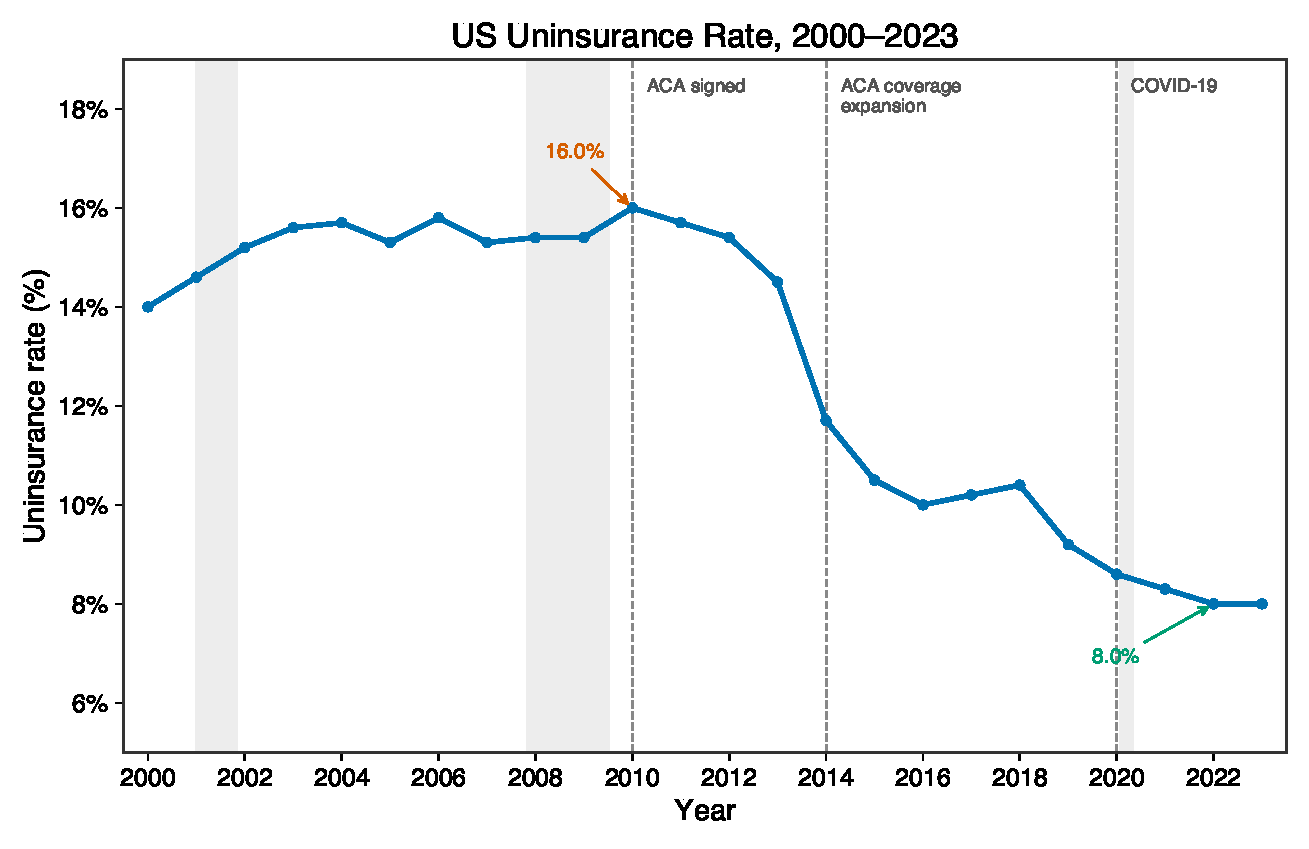
\includegraphics[height=0.58\textheight]{fig_overall_uninsurance.pdf}
\end{center}

\vspace{0.1cm}
\textbf{Headline:} high through the 2000s, then a sharp decline after the 2014 ACA coverage expansion.
\end{frame}

\begin{frame}{Figure 2: By Age Group}
\begin{center}
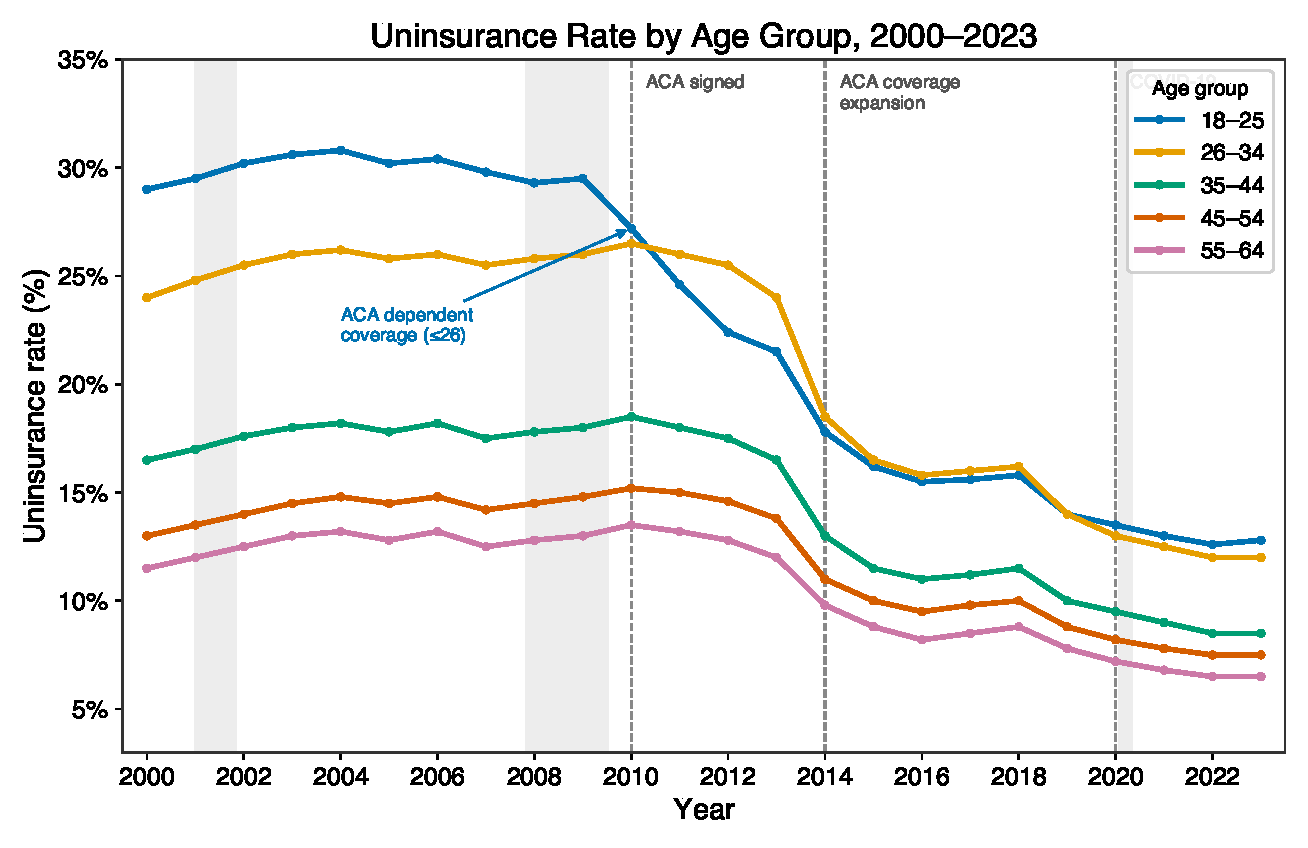
\includegraphics[height=0.58\textheight]{fig_uninsurance_by_age.pdf}
\end{center}

\vspace{0.1cm}
\textbf{Economic reading:} the life-cycle profile is steep, and the post-ACA drop is not uniform across ages.
\end{frame}

\begin{frame}{Figure 3: By Poverty Category}
\begin{center}
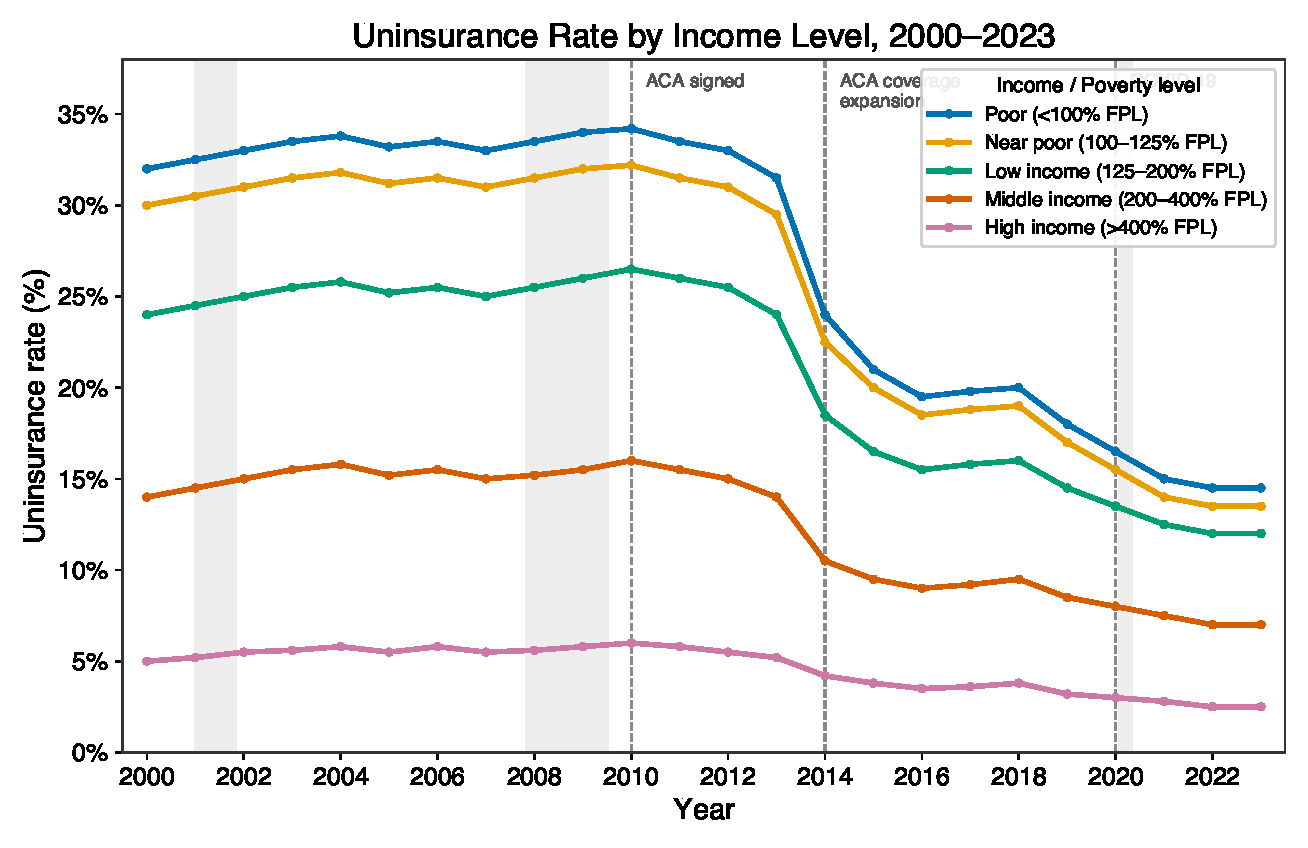
\includegraphics[height=0.57\textheight]{fig_uninsurance_by_poverty.pdf}
\end{center}

\vspace{0.1cm}
\textbf{Economic reading:} the largest levels and some of the largest gains are concentrated lower in the income distribution.
\end{frame}

\begin{frame}{Figure 4: By Race and Ethnicity}
\begin{center}
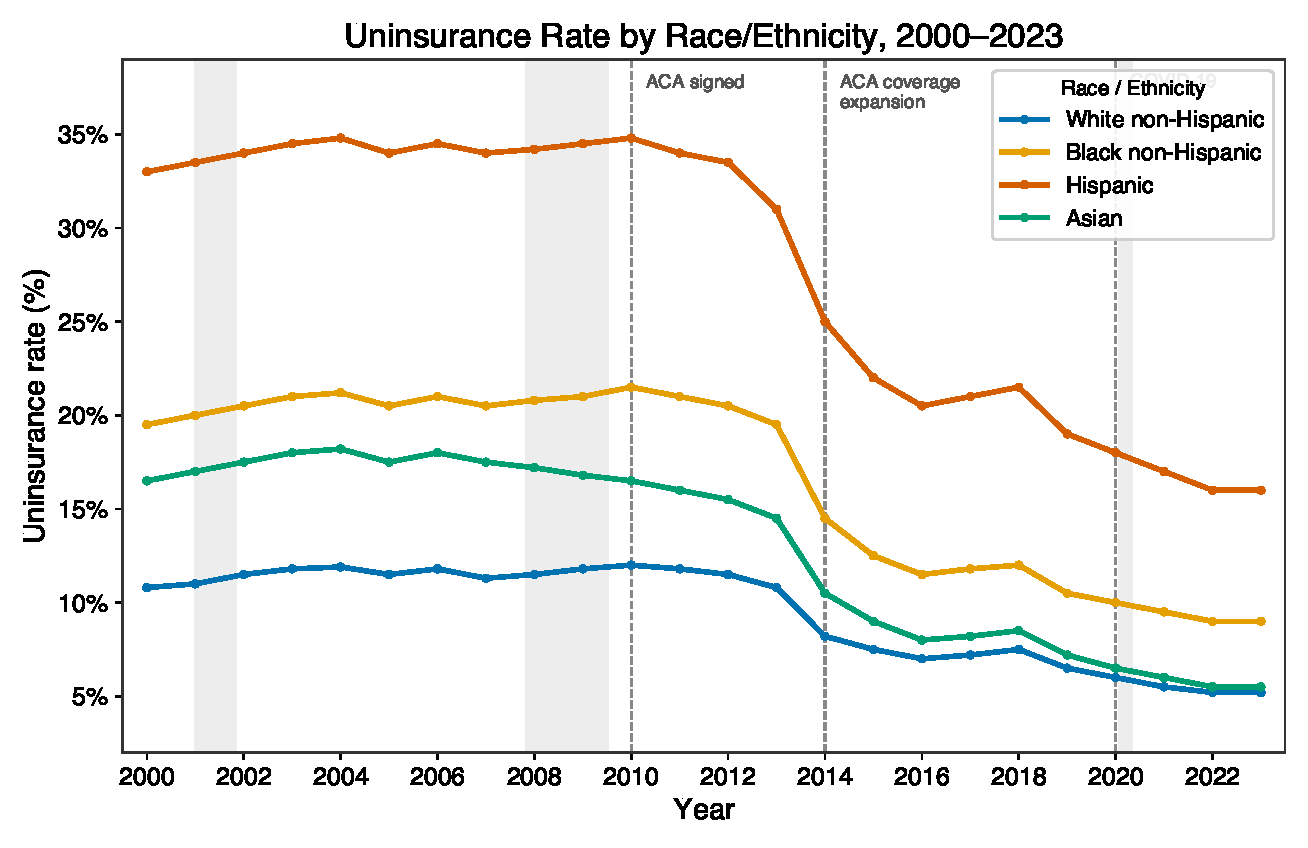
\includegraphics[height=0.58\textheight]{fig_uninsurance_by_race.pdf}
\end{center}

\vspace{0.1cm}
\textbf{Economic reading:} the ACA compresses disparities, but it does not erase them.
\end{frame}

\begin{frame}{Figures 5 and 6: Employment and Region}
\begin{columns}[T]
\begin{column}{0.49\textwidth}
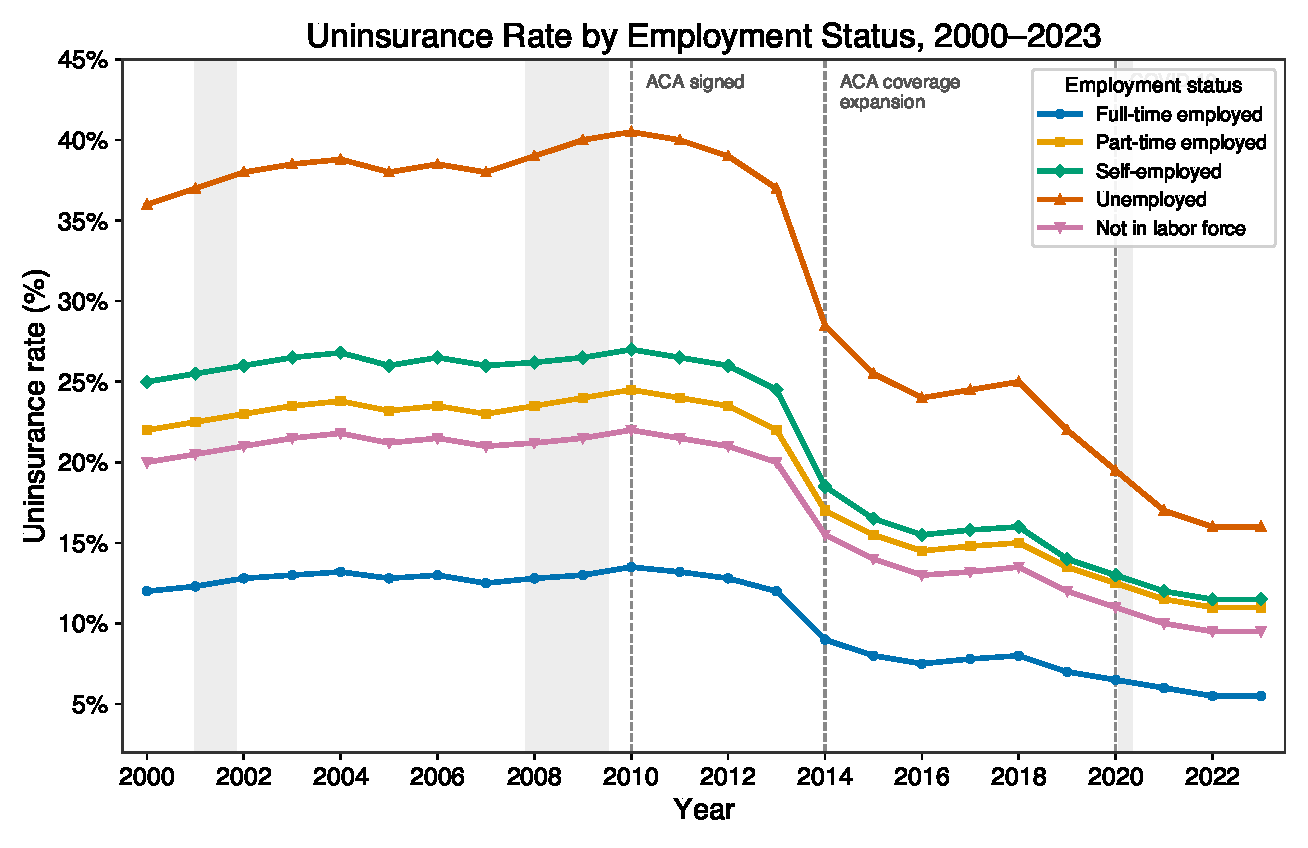
\includegraphics[width=\textwidth]{fig_uninsurance_by_employment.pdf}
\end{column}
\begin{column}{0.49\textwidth}
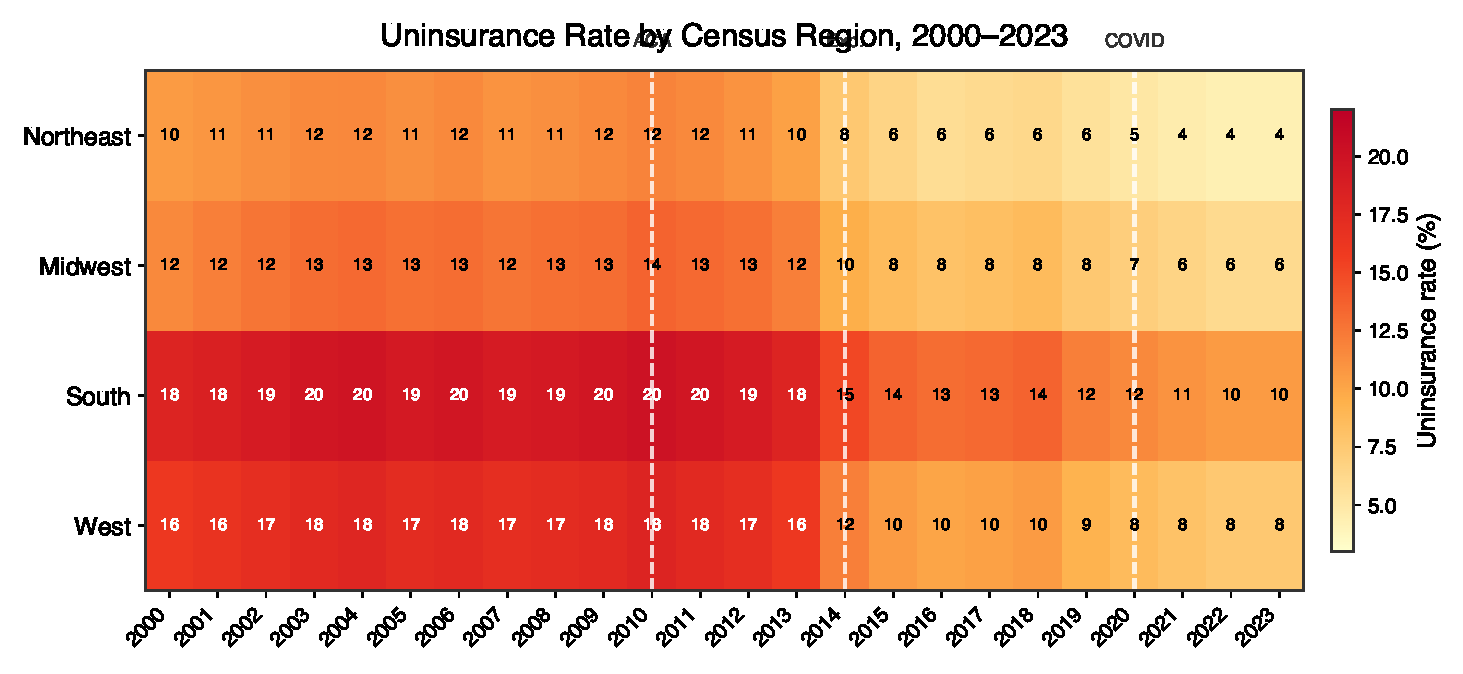
\includegraphics[width=\textwidth]{fig_uninsurance_heatmap.pdf}
\end{column}
\end{columns}

\vspace{0.15cm}
\textbf{Takeaway:} one pipeline can generate multiple cuts of the same policy story once the harmonized panel exists.
\end{frame}

\begin{frame}{What Claude Did vs.\ What Stayed Human}
\begin{columns}[T]
\begin{column}{0.48\textwidth}
\textbf{Agent}
\begin{itemize}
    \item downloaded files
    \item handled parsing obstacles
    \item built the crosswalk
    \item computed weighted statistics
    \item rendered figures
\end{itemize}
\end{column}
\begin{column}{0.48\textwidth}
\textbf{Economist}
\begin{itemize}
    \item chose the question
    \item specified the weights
    \item chose the subgroup cuts
    \item validated against benchmarks
    \item interpreted the policy story
\end{itemize}
\end{column}
\end{columns}
\end{frame}

\begin{frame}{Exercise A: Guided MEPS Lab}
\begin{itemize}
    \item keep the in-class lab short and structured
    \item students run the same three-prompt arc from the lecture
    \item success criteria:
    one merged file, weighted group-level CSVs, and at least three validated figures
    \item the notebook is the operational handout; the slides only carry the logic
\end{itemize}

\vspace{0.3cm}
\textbf{Pedagogical point:} the lab is about directing the agent and checking the output, not about typing code by hand.
\end{frame}


\end{document}
